\section{Конструкторская часть}
В данном разделе представлены требования к программному обеспечению, рассмотрены алгоритмы, выбранные для построения сцены

\subsection{Требования к программному обеспечению}

Программа должна предоставлять графический интерфейс с функционалом:
\begin{itemize}
	\item задать параметрические и спектральные характеристики, добавляемой модели многогранника;
	\item изменение положение модели многогранника в пространстве;
	\item изменение положение камеры и направления ее взгляда в пространстве;
	\item изменение характеристик модели многогранника.
\end{itemize}

Разработанное программное обеспечение должно соответствовать следующим требованиям:
\begin{itemize}
	\item источник света создается при запуске программы;
	\item нельзя иметь больше 1 камеры в пространстве;
	\item программа должна корректно обрабатывать ввод некорректных данных;
	\item все объекты создаются путем ввода его параметрических и спектральных характеристик.
\end{itemize}

\subsection{Описание структур данных}

Для формирования общего алгоритма синтеза изображения в данной программе, необходимо ввести определения использующихся в ней структур данных.
\begin{enumerate}
	\item Сцена представляет собой список с произвольным числом моделей, объект камеры и объект источника освещения.
	\item Модель многогранника включает в себя следующие данные:
	\begin{itemize}
		\item массив вершин фигуры;
		\item массив полигонов фигуры;
		\item массив векторов нормалей к вершинам;
		\item коэффициенты отражения и блеска поверхности;
		\item цвет поверхности;
		\item матрица аффинных преобразований.
	\end{itemize}
	\item Камера содержит:
	\begin{itemize}
		\item положение в пространстве;
		\item значения углов тангажа и рыскания,;
		\item систему координат камеры, задаваемую тремя ортогональными векторами;
		\item угол обзора и соотношение сторон экрана;
		\item цвет поверхности;
		\item границы пирамиды видимости.
	\end{itemize}
	\item Источник освещения включает: положение в пространстве и цвет источника.
\end{enumerate}

\subsection{Общий алгоритм построения изображения}

Алгоритм генерации изображения представлен на рисунке~\ref{fig:alg_scene}.
На вход подается геометрические характеристики моделей, камеры, источника, освещения, спектральные характеристики моделей и источника освещения.
На выход выдается результат построения буфера кадра сцены.

\begin{figure}[h]
	\centering
	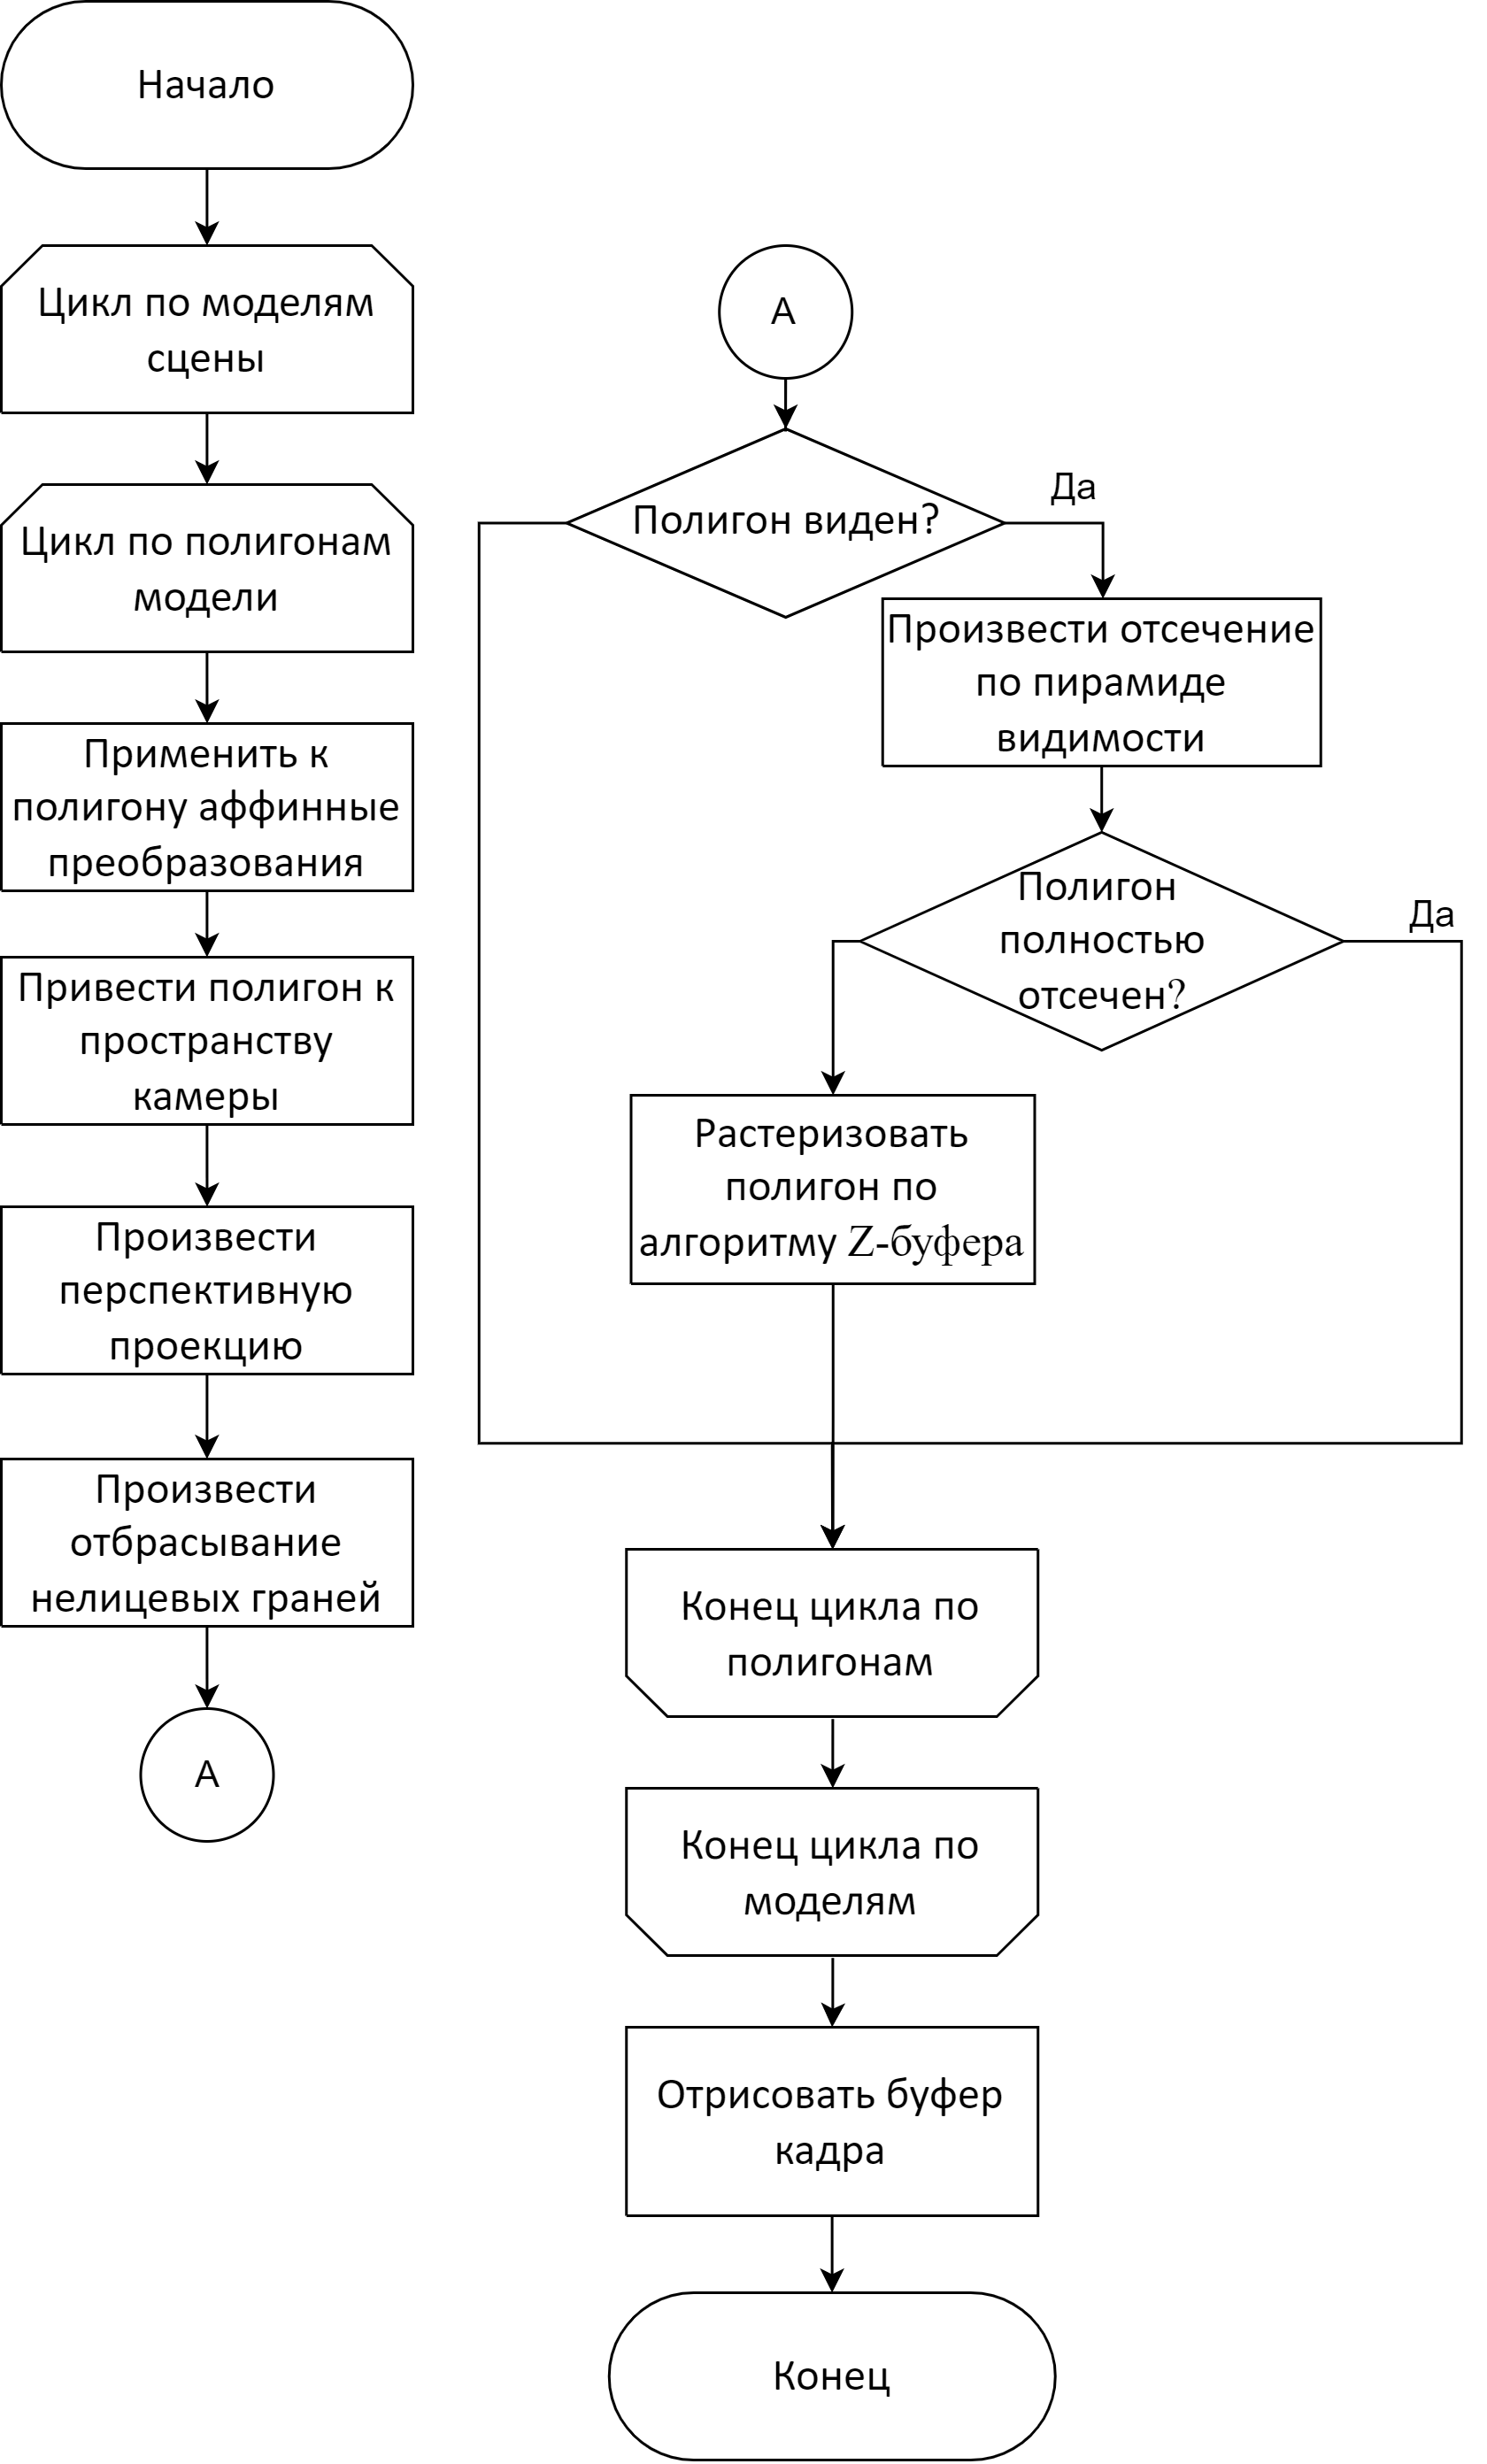
\includegraphics[width=0.8\textwidth]{img/alg_scene.png}
	\caption{Общая схема алгоритма синтеза изображения}
	\label{fig:alg_scene}
\end{figure}

\clearpage

\subsection{Аффинные преобразования}

В представленном алгоритме синтеза изображения первым этапом преобразования полигона пред его растеризацией является переход модели в мировое пространство. 
Такое действие осуществляется с помощью матриц аффинных преобразований~\cite{porevcg}.
В данном курсовом проекте над объектами возможно произвести следующие операции.

\begin{itemize}
	\item Поворот вокруг координатных осей описывается углом $\alpha$ и осью вращения.
	Матрица поворота имеет вид:
	\begin{itemize}
		\item вокруг оси OX:
		\begin{equation}
			\begin{pmatrix}
				1 	& 0 		  & 0 	       & 0 \\
				0 	& cos \alpha  & sin \alpha & 0 \\
				0	& -sin \alpha & cos \alpha & 0 \\
				0 	& 0 		  & 0          & 1
			\end{pmatrix}
		\end{equation}
		\item вокруг оси OY:
			\begin{equation}
			\begin{pmatrix}
				cos \alpha 	& 0 & -sin \alpha & 0 \\
				0 			& 1 & 0 		  & 0 \\
				sin \alpha	& 0 & cos \alpha  & 0 \\
				0 			& 0 & 0           & 1
			\end{pmatrix}
		\end{equation}
		\item вокруг оси OZ:
		\begin{equation}
			\begin{pmatrix}
				cos \alpha 	 & sin \alpha & 0 & 0 \\
				-sin \alpha  & cos \alpha & 0 & 0 \\
				0	 		 & 0		  & 1 & 0 \\
				0 			 & 0 		  & 0 & 1
			\end{pmatrix}
		\end{equation}
	\end{itemize}
	\item Перенос в трехмерном пространстве задается значения вдоль координатных осей OX, OY, OZ --- dx, dy, dz соответственно.
	Матрица переноса имеет вид:
	\begin{equation}
		\begin{pmatrix}
			1  & 0  & 0  & 0 \\
			0  & 1  & 0  & 0 \\
			0  & 0  & 1  & 0 \\
			dx & dy	& dz & 1
		\end{pmatrix}
	\end{equation}
\end{itemize}

\subsection{Приведение к пространству камеры}

Для перемещения по сцене используется камера, задаваемая точкой положения в пространстве, пирамидой видимости и собственной системой координат, которая состоит из трех ортогональных векторов.

Обозначим:
\begin{itemize}
	\item P --- положение камеры;
	\item D --- вектор взгляда;
	\item U --- вектор вверх;
	\item R --- вектор вправо.
\end{itemize}

Для перехода в пространство камеры выполняется в два этапа, указанные далее.
\begin{enumerate}
	\item Перенос полигона в отрицательную стороны от камеры на расстояние P с помощью матрицы переноса~\cite{palcing-camera}:
	\begin{equation}
		\begin{pmatrix}
			1  & 0  & 0  & 0 \\
			0  & 1  & 0  & 0 \\
			0  & 0  & 1  & 0 \\
			-Px & -Py & -Pz & 1
		\end{pmatrix}
	\end{equation}
	\item Преобразование полигона к системе координат камеры при помощи матрицы поворота~\cite{palcing-camera}:
	\begin{equation}
		\begin{pmatrix}
			Rx  & Ux  & Dx  & 0 \\
			Ry  & Uy  & Dy  & 0 \\
			Rz  & Uz  & Dz  & 0 \\
			0   & 0   & 0   & 1
		\end{pmatrix}
	\end{equation}
\end{enumerate}

Управление камеры производится с помощью изменения углом Эйлера.
Обозначим $\alpha$ --- угол поворота вокруг оси ОУ (тангаж) и  $\beta$ --- угол поворота вокруг оси OX (рыскание).
Тогда координаты вектора направления камеры можно вычислить по следующим формулам:
\begin{equation}
	D_x = cos(\alpha) \cdot cos(\beta)
\end{equation}
\begin{equation}
	D_y = sin(\alpha)
\end{equation}
\begin{equation}
	D_z = cos(\alpha) \cdot sin(\beta)
\end{equation}

\subsection{Перспективная проекция}

После перехода в пространство камеры необходимо спроецировать полигон на картинную плоскость.
В данном курсовом проекте используется перспективная проекция.
Обозначим:
\begin{itemize}
	\item $zoom_x$ --- приближение по X;
	\item $zoom_y$ --- приближение по Y;
	\item $R$ --- соотношение сторон экрана;
	\item $F$ --- расстояние от камеры до задней грани пирамиды видимости;
	\item $N$ --- расстояние от камеры до передней грани пирамиды видимости;
	\item $\gamma$ --- вертикальный угол обзора.
\end{itemize}
Увеличение объектов по координатам X и Y можно вычислить по формулах:
\begin{equation}
	zoom_y = \frac{1}{tg(\gamma / 2)}
\end{equation}
\begin{equation}
	zoom_x = \frac{zoom_y}{R}
\end{equation}

Для перехода в пространство отсечения используется матрица перспективной проекции:
\begin{equation}
	\begin{pmatrix}
		zoom_x  & 0  & 0  & 0 \\
		0   & zoom_y  & 0  & 0 \\
		0   & 0   & \frac{F + N}{F - N}  & 1 \\
		0   & 0   & \frac{-2 \cdot F \cdot N}{F - N}  & 0
	\end{pmatrix}
\end{equation}

\subsection{Отбрасывание невидимых граней}

С помощью отбрасывания нелицевых граней моделей при построении изображения можно существенно сократить временные затраты, так как не полигоны, невидимые по отношению к камере, растеризоваться не будут.
Для определения видимости грани требуется использовать формулу:
\begin{equation}
	(\overrightarrow{N}, \overrightarrow{V}) = \begin{cases}
		 \geq 0,~\text{если грань невидима} \\
		 < 0,~\text{если грань видима}
	\end{cases},
\end{equation}
где $\overrightarrow{N}$ --- вектор внешней нормали к грани модели, $\overrightarrow{V}$ --- вектор от камеры до любой точки грани.

\subsection{Отсечение по пирамиде видимости}

Отсечение полигона по пирамиде видимости решает две задачи:
\begin{enumerate}
	\item удаление полигонов, лежащих за камерой, но проецируемых на картинную плоскость в перевернутом виде;
	\item сокращение времени на растеризацию полигонов за счет удаления их невидимых частей.
\end{enumerate}

Для выполнения операции отсечения в данном курсовом проекте использовался алгоритм Сазерленда-Ходжмана~\cite{roders}. Согласно рисунку~\ref{saz-hodj} его идея состоит в том, чтобы последовательно отсекать полигон относительно каждой грани пирамиды видимости до тех пор, пока полигон не будет отсечен полностью либо пока все грани не будут пройдены.

\begin{figure}[h]
	\centering
	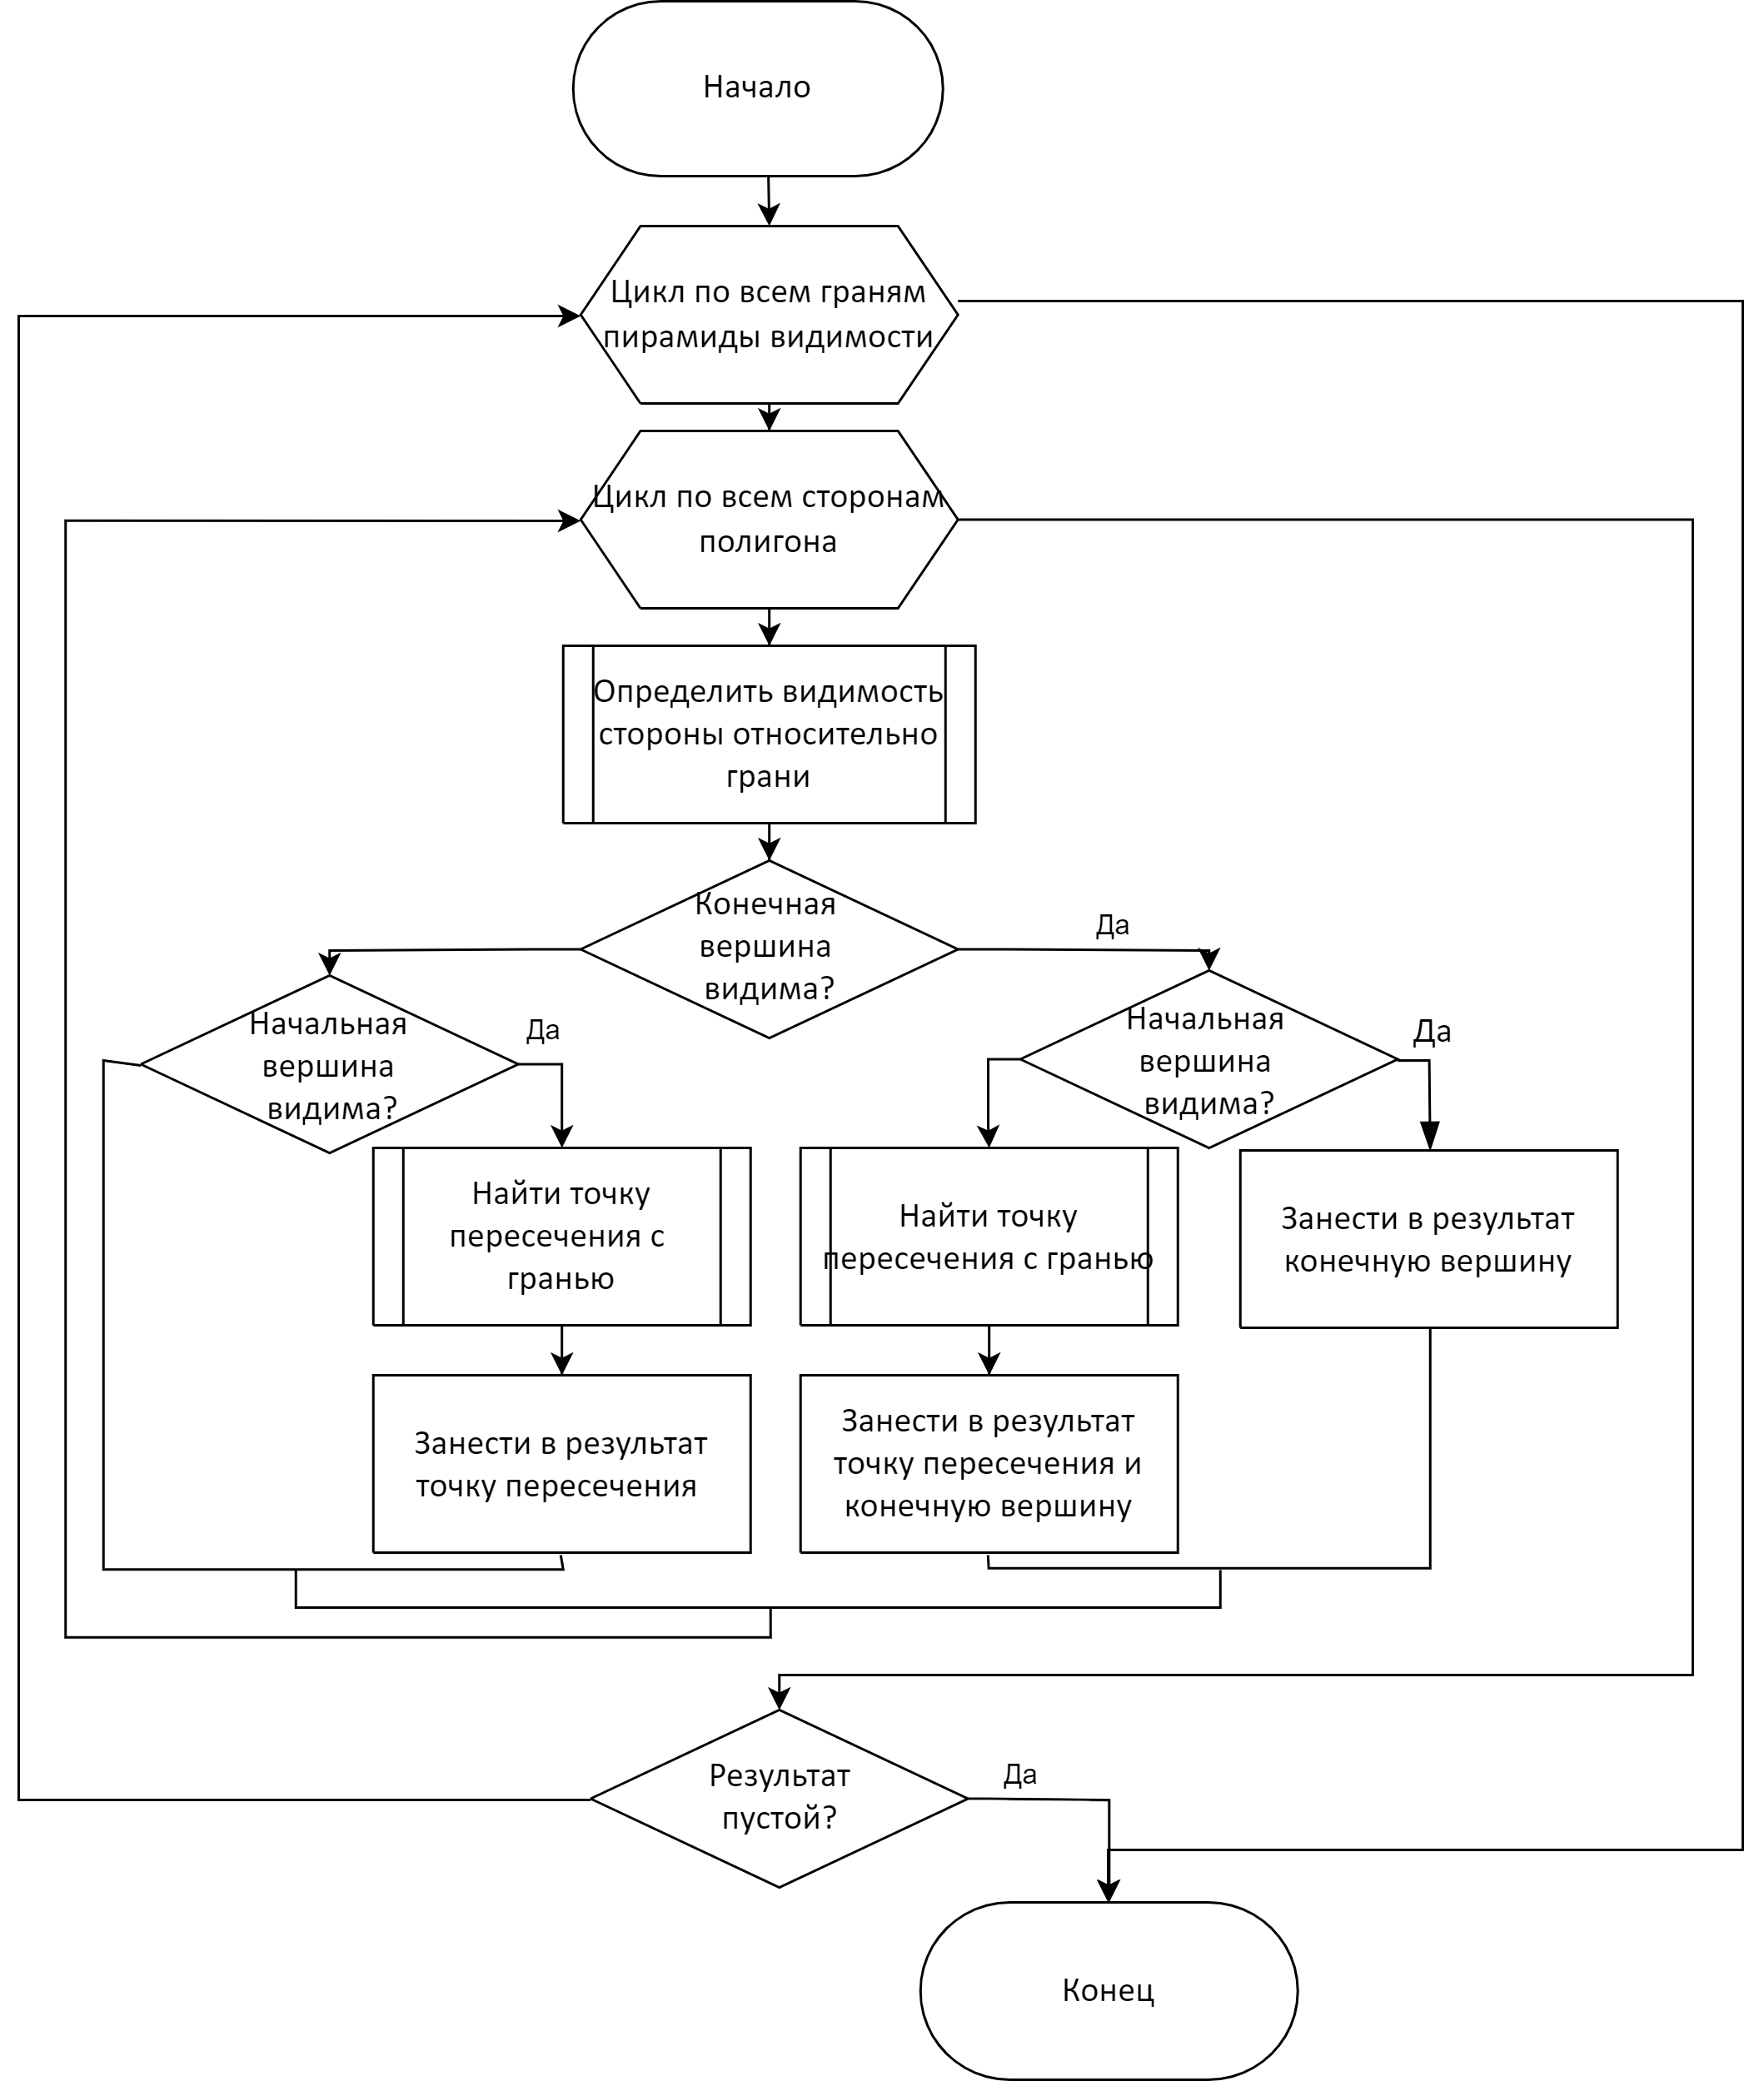
\includegraphics[width=0.9\textwidth]{img/sаz-hodj.png}
	\caption{Схема алгоритма Сазерленда-Ходжмана}
	\label{fig:saz-hodj}
\end{figure}

\clearpage

\subsection{Алгоритм Z-буфера}

Для растеризации треугольного полигона сначала необходимо найти ограничивающий его прямоугольник, в котором это полигон содержится. 
Это делается для того, чтобы не тратить время на растеризацию пикселей, не являющихся частью полигона.
Затем для каждого пиксела ограничивающего прямоугольника находятся его барицентрические координаты относительно вершин полигона.

Пусть $A, B, C$ – вершины грани, $P$ – пиксель внутри ограничивающего прямоугольника.
Площадь треугольника можно найти по следующей формуле:
\begin{equation}
	square = (A_y - C-y) \cdot (B_x - C_x) + (B_y - C_y) \cdot (C_x - A_x)
\end{equation}

Тогда барицентрические координаты пиксела равны:

\begin{equation}
	\alpha=\frac{\left(P_y-C_y\right)\cdot\left(B_x-C_x\right)+\left(B_y-C_y\right)\cdot\left(C_x-P_x\right)}{square}
\end{equation}	

\begin{equation}
	\beta=\frac{\left(P_y-A_y\right)\cdot\left(C_x-A_x\right)+\left(C_y-A_y\right)\cdot\left(A_x-P_x\right)}{square}
\end{equation}

\begin{equation}
	\gamma=1-\ \alpha-\ \beta
\end{equation}

В случае, если хоть одна из барицентрических координат отрицательна, то пиксель лежит вне полигона. Если пиксель лежит внутри треугольника, то найти значение его глубины можно по следующей формуле:

\begin{equation}
	z=\frac{1}{\frac{\alpha}{A_z}+\frac{\beta}{B_z}+\frac{\gamma}{C_z}}
\end{equation}

Затем производится сравнение значения глубины точки со значением глубины из Z-буфера. Если глубина пикселя меньше, значит он лежит ближе к камере и должен быть растеризован. Происходит вычисление интенсивности пикселя, его значение заносится в буфер кадра, а в Z-буфер заносится значение глубины пиксела. Полная схема алгоритма Z-буфера представлена на 
рисунке~\ref{fig:z-buffer}.

\begin{figure}[h]
	\centering
	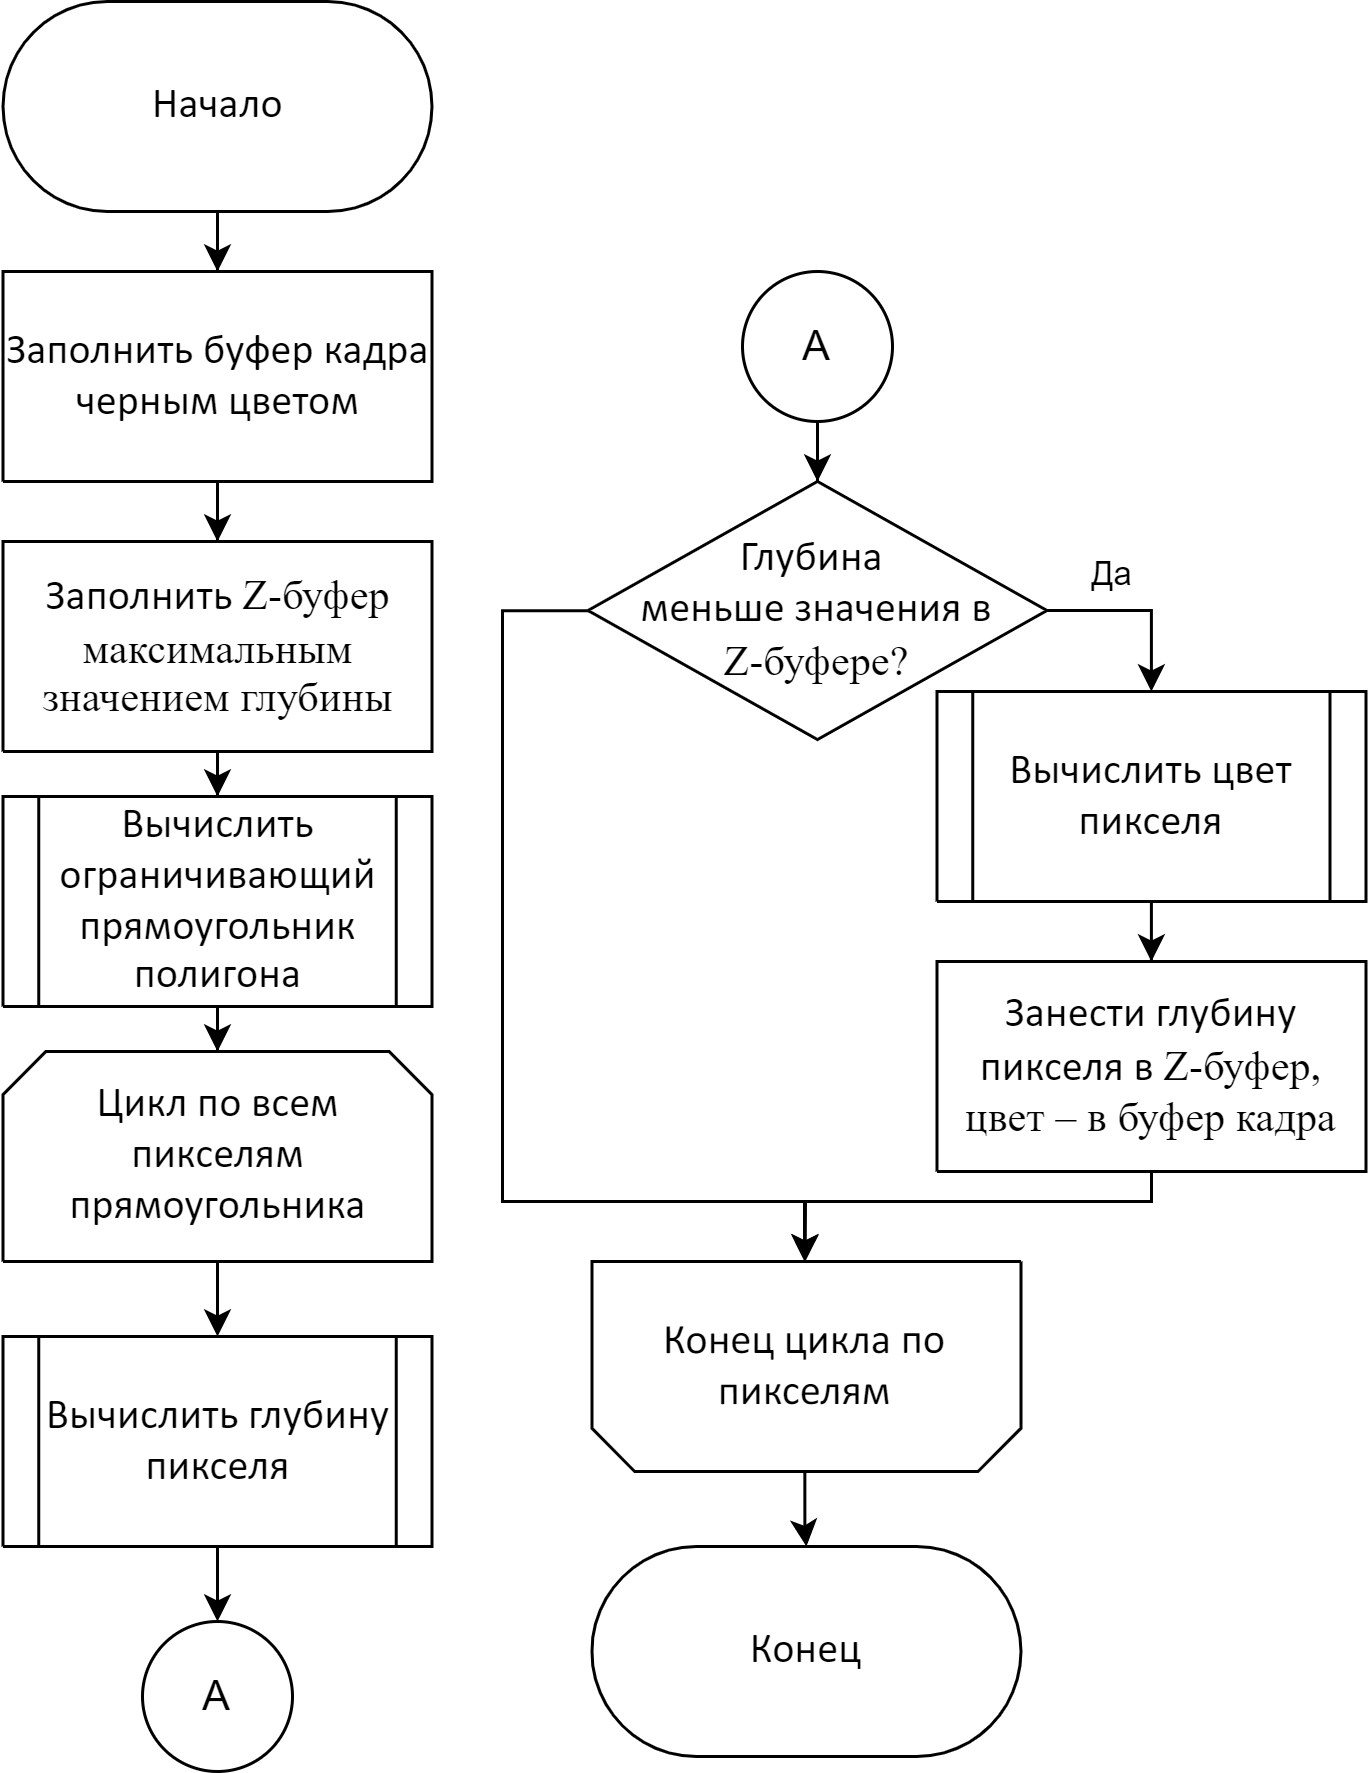
\includegraphics[width=0.8\textwidth]{img/alg-z-buffer.png}
	\caption{Схема алгоритма Z-буфера}
	\label{fig:z-buffer}
\end{figure}

\subsection*{Вывод}
Были описаны требования к программному обеспечению, структур данных, алгоритмы для построения сцены в пространстве изображения, изменения положения объекта в пространстве, построение камеры и ее проекций.